\documentclass[xetex,table]{beamer}

\usepackage[autostyle]{csquotes}
\usepackage{hyperref}
\usepackage{color}
\usepackage{setspace}
\usepackage{listings}
\usepackage{minted}

\usetheme{metropolis}

\usemintedstyle{perldoc}
\definecolor{codebackground}{rgb}{0.96,0.96,0.75}

\title{ARM64 + FPGA and more:\\Linux on the Xilinx ZynqMP}
\subtitle{Opportunities and challenges from a powerful and complex chip}
\author{Luca Ceresoli, AIM Sportline\\
  \href{mailto:luca@lucaceresoli.net}{\tt luca@lucaceresoli.net}\\
  \url{http://lucaceresoli.net}
}
\date{FOSDEM 2018}

\begin{document}

\maketitle

\begin{frame}{About me}
  \begin{columns}
    \column{0.4\textwidth}
    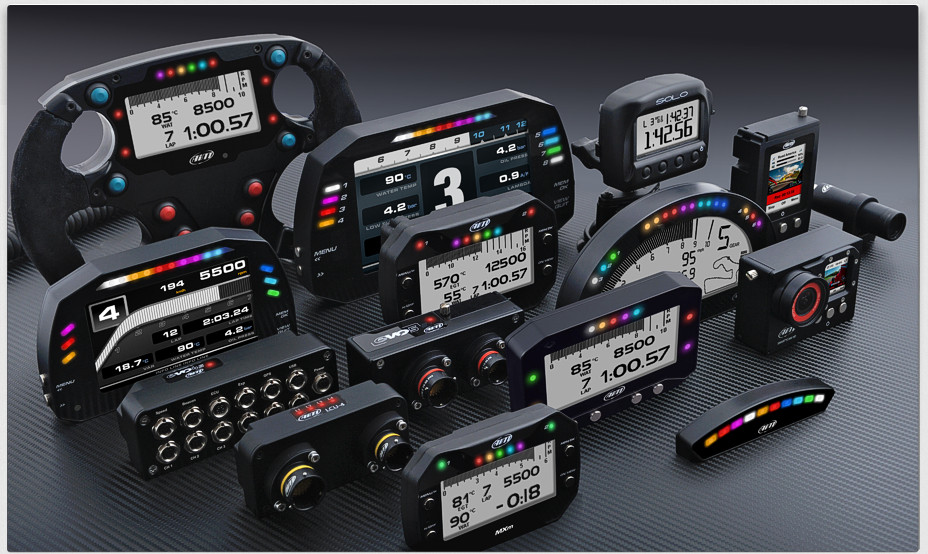
\includegraphics[width=\textwidth]{../common/images/aim-products.jpg}

    \column{0.6\textwidth}
    \begin{itemize}
    \item Embedded Linux engineer\\
      at AIM Sportline\\
      {\footnotesize\url{http://www.aim-sportline.com/}}
      \begin{itemize}
      \item Develop real products on custom hardware
      \item Kernel, bootloader, drivers
      \item Integration, build system
      \end{itemize}
    \item Open source enthusiast
      \begin{itemize}
      \item Contributor to Buildroot and a few other projects
      \end{itemize}
    \end{itemize}
  \end{columns}
\end{frame}

\begin{frame}{Agenda}
  \begin{itemize}
  \item Introduction
  \item Development tools
  \item Linux on your FPGA design
  \item Booting
  \item GPU
  \item Video Codec Unit
  \item Conclusion
  \end{itemize}
\end{frame}

\section{Introduction}

\begin{frame}{SoC+FPGA: what is it?}
  \begin{itemize}
  \item A SoC and an FPGA on a single chip
  \item Connected on-chip
  \item Other technologies:
    \begin{itemize}
    \item 2 chips: a SoC and an FPGA, connected via pins
    \item An FPGA with a synthesized ``soft core'' CPU
    \end{itemize}
  \item A good introduction to SoC+FPGA:\\
    Introduction to SoC+FPGA, Marek Vašut, ELC-E 2017\\
    {\footnotesize\url{https://elinux.org/images/e/ed/Elce-2017-socfpga.pdf}}\\
    {\footnotesize\url{https://youtu.be/R3gJhnGjjWY}}
  \end{itemize}
\end{frame}

\begin{frame}{Current Linux-capable SoC+FPGAs}
  \begin{itemize}
  \item Xilinx
    \begin{itemize}
    \item 1st generation: Zynq 7000
    \item 2nd generation: Zynq UltraScale+ MPSoC (aka ZynqMP)
    \end{itemize}
  \item Intel (Altera)
    \begin{itemize}
    \item 1st generation: Cyclone V and Arria V
    \item 2nd generation: Stratix 10
    \end{itemize}
  \end{itemize}
\end{frame}

\begin{frame}{ZynqMP block diagram (simplified)}
  \begin{center}
    \includegraphics[height=0.9\textheight]{images/block-diagram.pdf}
  \end{center}
\end{frame}

\section{Development tools}

\begin{frame}{Documentation}
  \begin{itemize}
  \item A lot of documentation by Xilinx
  \item Start from the Xilinx ZynqMP Documentation hub\\
    {\tiny\url{https://www.xilinx.com/support/documentation-navigation/design-hubs/dh0070-zynq-mpsoc-design-overview-hub.html}}
  \end{itemize}
\end{frame}

\begin{frame}[standout]
  FPGA development
\end{frame}

\begin{frame}{FPGA Development Tools --- Xilinx}
  Xilinx Vivado Design Suite
  \begin{itemize}
  \item Vivado: design FPGA to bitstream
  \item XSDK: eclipse IDE for firmware development
  \item Runs on Linux
  \item Has a zero-cost version (has most features, not the advanced
    ones)
  \item Closed source, huge, has some bugs and issues
  \end{itemize}
\end{frame}

\begin{frame}{FPGA Development Tools --- Open source}
  \begin{itemize}
  \item No open source FPGA toolchain available
  \item Bitstream reverse engineering in progress
    (\url{https://symbiflow.github.io/})
  \item On why FPGA open source toolchains matter:
    {\footnotesize\url{https://blog.elphel.com/2013/10/fpga-is-for-freedom/}}
  \end{itemize}
\end{frame}

\begin{frame}[standout]
  BSP components
\end{frame}

\begin{frame}{U-Boot}
  \begin{itemize}
  \item Xilinx is active in mainlining
  \item Discussion: \texttt{U-Boot@lists.denx.de}
  \item Mainline U-Boot enough to boot
  \item Newer boards are available at
    \url{https://github.com/xilinx/u-boot-xlnx}
  \item Note: ZynqMP cannot boot U-Boot the ``normal'' way, see {\em
    Booting} section later
  \end{itemize}
\end{frame}

\begin{frame}{Linux kernel}
  \begin{itemize}
  \item Xilinx is active in mainlining
  \item Discussion: \texttt{linux-arm-kernel@lists.infradead.org}
  \item Mainline Linux: partially implemented
  \item Development in progress at
    \url{https://github.com/xilinx/linux-xlnx}\\
    (especially the \texttt{master} branch)
    \begin{itemize}
      \item ``Hard'' silicon features
      \item Recent UltraScale+ IPs from Xilinx, mostly video-related
    \end{itemize}
  \end{itemize}
\end{frame}

\begin{frame}[standout]
  Build system
\end{frame}

\begin{frame}{Available workflows}
  Typical ways to build the software stack for Xilinx products:
  \begin{itemize}
  \item The {\bf ``Xilinx workflow''}
    \begin{itemize}
    \item Officially supported by Xilinx
    \end{itemize}
  \item The {\bf ``Community workflow''}
    \begin{itemize}
    \item Similar to other open source projects
    \item Supported by the community (with Xilinx contributions)
    \end{itemize}
  \item Other/mixed workflows
  \end{itemize}
\end{frame}

\begin{frame}{The Xilinx workflow}
  \begin{itemize}
  \item FPGA: Vivado
  \item Baremetal and bootloaders: XSDK
  \item Petalinux
    \begin{itemize}
    \item A Xilinx-specific embedded build system
    \item Nowadays internally uses Yocto
    \end{itemize}
  \item Yocto layers on \url{https://github.com/xilinx}
    \begin{itemize}
    \item A {\tt meta-xilinx-bsp} fork
    \item {\tt meta-xilinx-tools} to use Xilinx tools during the build
    \item {\tt meta-petalinux}: a distro layer
    \item Note: these layers will soon be moved to subdirs of {\tt
      meta-xilinx}
  \end{itemize}
  \end{itemize}
\end{frame}

\begin{frame}{The Community workflow}
  \begin{itemize}
  \item FPGA: Vivado
  \item A little bit of XSDK
  \item Yocto {\tt meta-xilinx-bsp} layer\\
    {\footnotesize\url{https://git.yoctoproject.org/cgit/cgit.cgi/meta-xilinx/}}
    subdir {\tt meta-xilinx-bsp}
    \begin{itemize}
      \item Until a few weeks ago: in the top dir, and called {\tt meta-xilinx}
  \end{itemize}
  \item Goal: follow the common practices in FOSS/Yocto
  \item Not all features supported
  \end{itemize}
\end{frame}

\begin{frame}{Other resources}
  \begin{itemize}
  \item meta-xilinx mailing list
    \begin{itemize}
    \item {\footnotesize\url{https://lists.yoctoproject.org/listinfo/meta-xilinx}}
    \item Discussion on the Yocto layers
    \item Also for general discussion about Linux on Xilinx
      hardware
    \end{itemize}
  \item {\small\url{https://github.com/topic-embedded-products/meta-topic}}
    \begin{itemize}
    \item Support for boards by Topic Embedded
    \item But has very useful code (see {\em Booting} section later)
    \end{itemize}
  \end{itemize}
\end{frame}

\begin{frame}{Buildroot}
  \begin{itemize}
  \item Work in progress
  \item Patches to add basic support under discussion on the Buildroot
    mailing-list
  \end{itemize}
\end{frame}

\section{Linux on your FPGA design}

\begin{frame}{Build your own SoC!}
  \begin{itemize}
  \item FPGA $\leftrightarrow$ CPU interface is AXI4
  \item AXI = Advanced eXtensible Interface (part of AMBA)
  \item Peripherals in FPGA are accessible on the physical address
    space
    \begin{itemize}
    \item Like hard peripherals and traditional SoCs
    \end{itemize}
  \end{itemize}
\end{frame}

\begin{frame}{Typical workflow}
  \begin{itemize}
  \item Workflow with Vivado
    \begin{enumerate}
    \item IP integration
    \item Address editor
    \item Constraints
    \end{enumerate}
  \end{itemize}
\end{frame}

\begin{frame}[standout]
  Step 1: IP integration
\end{frame}

\begin{frame}{Vivado: block design}
  \center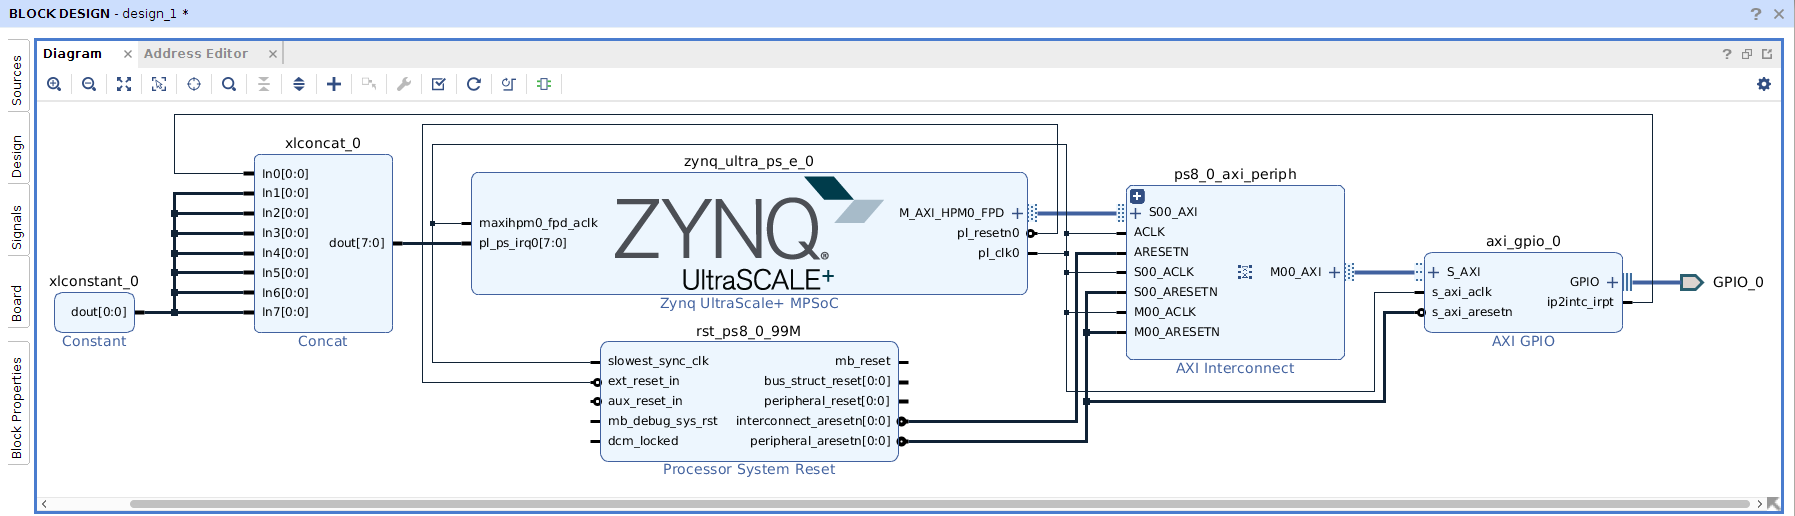
\includegraphics[width=1.0\textwidth]{images/block-design.png}
\end{frame}

\begin{frame}{Vivado: customize the PS block}
  \center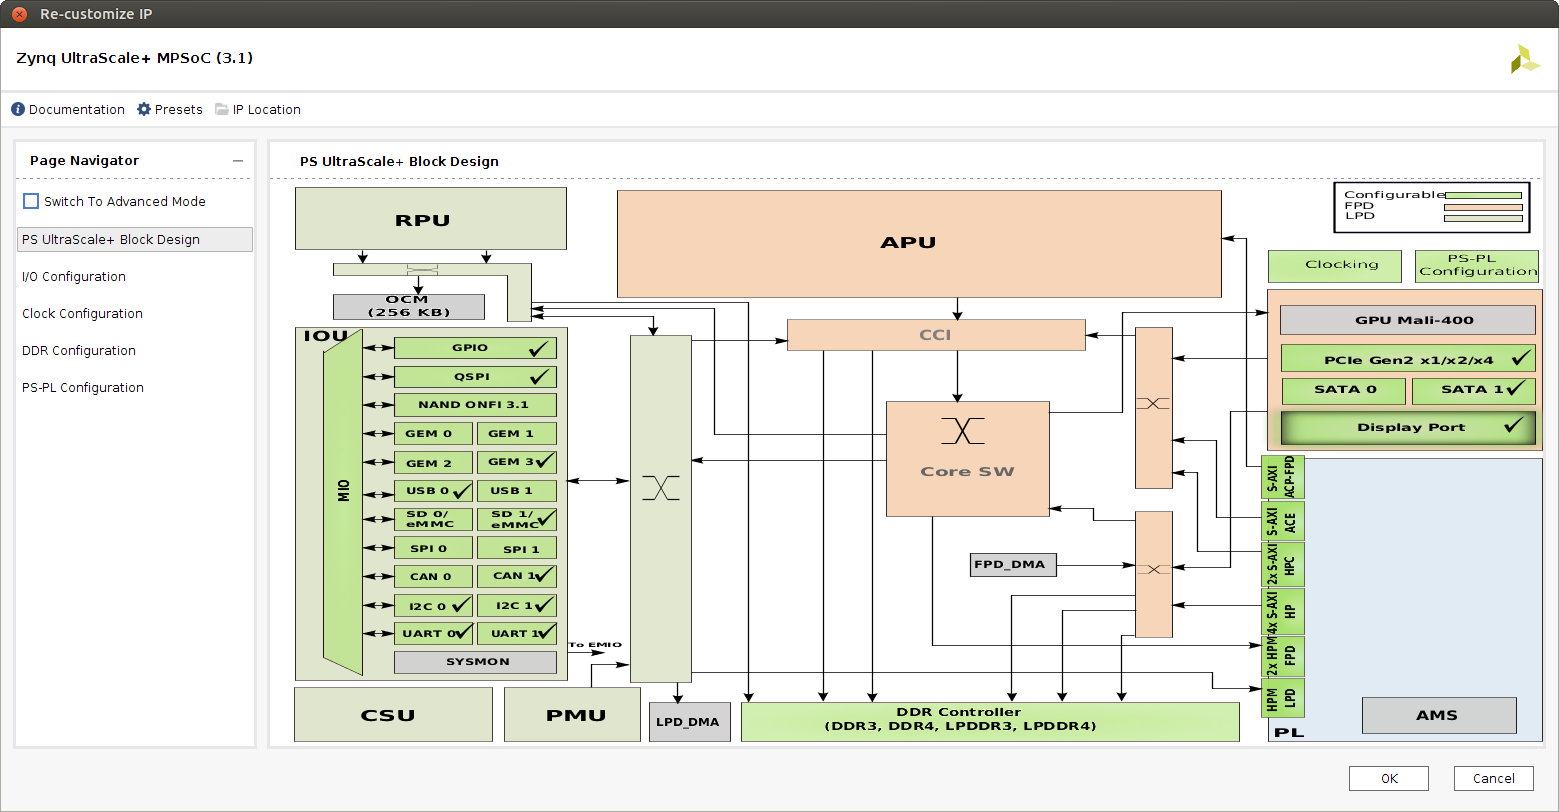
\includegraphics[width=1.0\textwidth]{images/customize-ps.png}
\end{frame}

\begin{frame}{Vivado: customize an IP block}
  \center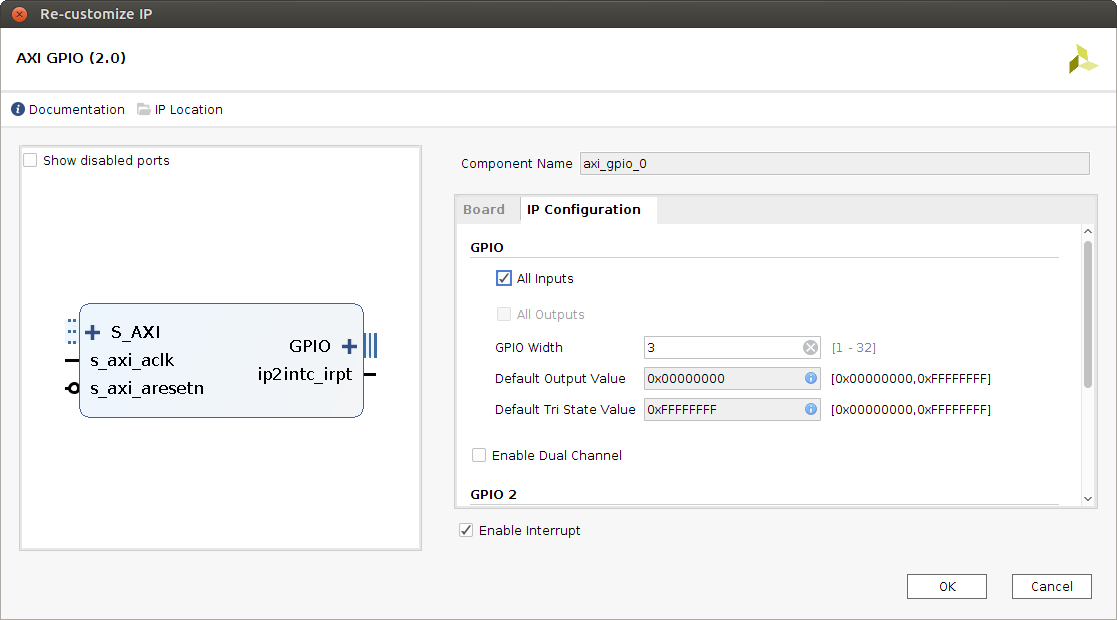
\includegraphics[width=1.0\textwidth]{images/customize-gpio.png}
\end{frame}

\begin{frame}[fragile]{Linux: instantiate a device}
  \begin{columns}
    \column{0.4\textwidth}
    \center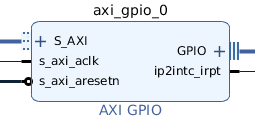
\includegraphics[height=0.2\textheight]{images/block-design-gpio.png}

    \column{0.6\textwidth}
    Linux drivers for Xilinx IPs:
    \href{http://www.wiki.xilinx.com/Linux+Drivers}{\tt wiki.xilinx.com/Linux+Drivers}
  \end{columns}

  \begin{minted}[bgcolor=codebackground,frame=single,autogobble,fontsize=\small]{perl}
  gpio: gpio@a0000000 {
    #gpio-cells = <2>;
    compatible = "xlnx,xps-gpio-1.00.a";
    gpio-controller;
    xlnx,gpio-width = <3>;
    xlnx,all-inputs = <1>;
    /*...*/
  };
  \end{minted}
\end{frame}

\begin{frame}[fragile]{Vivado: interrupts}
  \center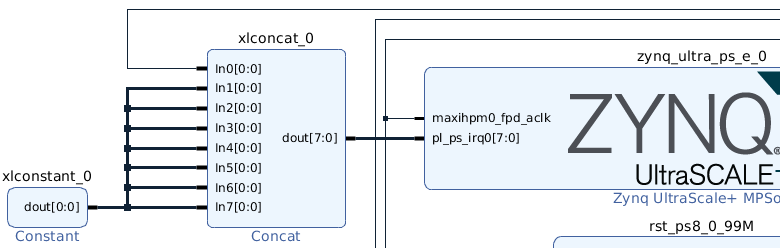
\includegraphics[width=1.0\textwidth]{images/block-design-interrupt.png}
\end{frame}

\begin{frame}[fragile]{Linux: interrupts}
  \begin{minted}[bgcolor=codebackground,frame=single,autogobble,fontsize=\small]{perl}
  #include <dt-bindings/interrupt-controller/arm-gic.h>
  #include "zynqmp-irqs.dtsh" // (*)

  gpio: gpio@a0000000 {
    #gpio-cells = <2>;
    compatible = "xlnx,xps-gpio-1.00.a";
    gpio-controller;
    interrupt-parent = <&gic>;
    interrupts = <GIC_SPI PL_PS_GRP0_IRQ_0
                  IRQ_TYPE_LEVEL_HIGH>;
    /*...*/
  };
  \end{minted}

  \footnotesize (*) From
  \href{https://github.com/xilinx/qemu-devicetrees/blob/master/zynqmp-irqs.dtsh}{\tt github.com/xilinx/qemu-devicetrees/blob/master/}
\end{frame}

\begin{frame}[standout]
  Step 2: Address editor
\end{frame}

\begin{frame}{Vivado: Address editor}
  \center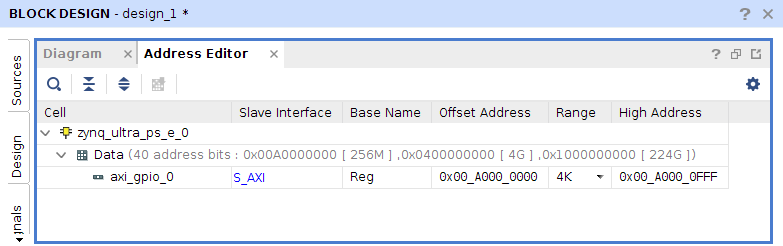
\includegraphics[width=1.0\textwidth]{images/address-editor.png}
\end{frame}

\begin{frame}[fragile]{Linux: address map}
  \begin{minted}[bgcolor=codebackground,frame=single,autogobble,fontsize=\small]{perl}
  gpio: gpio@a0000000 {
    #gpio-cells = <2>;
    compatible = "xlnx,xps-gpio-1.00.a";
    gpio-controller;
    reg = <0x0 0xa0000000 0x0 0x10000>;
    /*...*/
  };
  \end{minted}
\end{frame}

\begin{frame}[standout]
  Step 3: Constraints
\end{frame}

\begin{frame}{Vivado: constraints}
  \begin{itemize}
  \item Connect nets to pins: placement, IO standard, pull-up/down\dots
  \item No visible effect in Linux
  \end{itemize}

  \center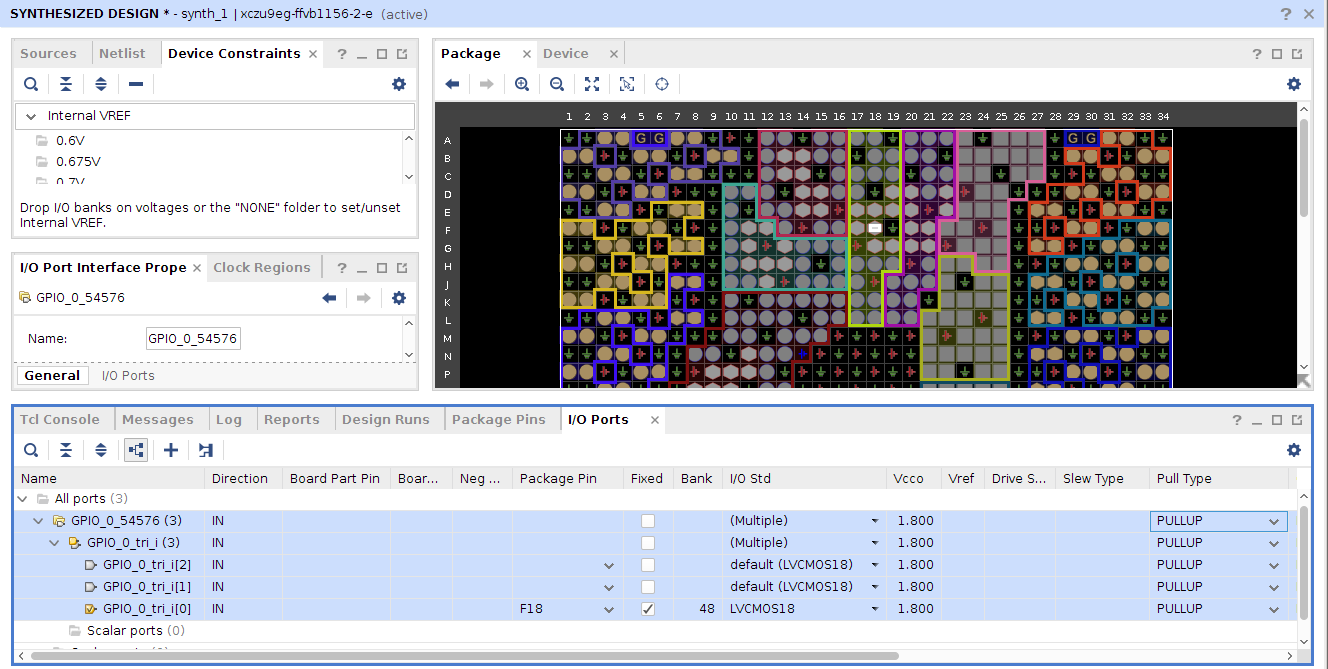
\includegraphics[width=1.0\textwidth]{images/pin-assignment.png}
\end{frame}

\section{Booting}

\begin{frame}{Simple ARM32 booting}
  \begin{itemize}
    \item Good old simple booting on ARM32:
    \begin{enumerate}
    \item Boot ROM loads SPL into internal RAM
    \item SPL initializes SDRAM, loads U-Boot
    \item U-Boot loads kernel
    \end{enumerate}
  \item But waking up in an ARM64 world is much more complex\dots
  \end{itemize}
\end{frame}

\begin{frame}{The Platform Management Unit (PMU)}
  \begin{columns}
    \column{0.55\textwidth}
  \begin{itemize}
  \item Duties:
    \begin{itemize}
    \item Power gates peripherals, power islands, power domains
    \item Clock gates peripherals
    \end{itemize}
  \item Can't boot without it
  \item Similar to other ARM64 boards
    \begin{itemize}
    \item E.g. the
      \href{https://developer.arm.com/products/system-design/development-boards/juno-development-board}{ARM
        Juno board}
    \end{itemize}
  \end{itemize}
  \column{0.45\textwidth}
    \includegraphics[width=\textwidth]{images/block-diagram.pdf}
  \end{columns}
\end{frame}

\begin{frame}{PMU firmware}
  \begin{itemize}
  \item PMU is a Microblaze core with 128 kB RAM
  \item Executes a firmware that {\em can} be reprogrammed
    \begin{itemize}
    \item But the one in ROM is not enough, so it {\em must} be
      reprogrammed
    \item Source at \url{https://github.com/xilinx/embeddedsw}
    \item {\tt meta-xilinx-bsp} {\tt master} can build it (not the
      Xilinx branches)
    \end{itemize}
  \item The PMUFW needs a {\em configuration object}
    \begin{itemize}
    \item Tells which master (CPU) owns which slave (peripheral)
    \item Depends on how the hardware is configured in Vivado
    \end{itemize}
  \end{itemize}
\end{frame}

\begin{frame}{ARM Trusted Firmware}
  A secure monitor reference implementation

   \begin{center}
    \includegraphics[height=0.7\textheight]{images/pm-layers.pdf}
  \end{center}
\end{frame}

\begin{frame}[standout]
   Booting --- The Xilinx workflow
\end{frame}

\begin{frame}{Boot sequence}
  \begin{center}
    \includegraphics[width=\textwidth]{images/boot-sequence-fsbl.pdf}
  \end{center}
\end{frame}

\begin{frame}{Building the pieces}
  \begin{center}
    \includegraphics[height=0.9\textheight]{images/build-xilinx.pdf}
  \end{center}
\end{frame}

\begin{frame}{Pros and cons}
    Pros
    \begin{itemize}
    \item The Xilinx tools make it easy
    \item FSBL is easy to understand and debug
    \end{itemize}

    Cons
    \begin{itemize}
    \item FSBL is slow (\textasciitilde{}3 seconds to load a 4 MB FPGA
        bitstream)
    \item The Xilinx tools: big and heavy, hard to automate
    \item Proprietary {\tt bootgen} tools needed to generate BOOT.BIN
    \item Non-standard (w.r.t. other SoCs)
    \end{itemize}
\end{frame}

\begin{frame}[standout]
   Booting --- The Community workflow
\end{frame}

\begin{frame}{FSBL \textrightarrow{} U-Boot SPL}
  Can U-Boot SPL replace Xilinx FSBL?
  \begin{itemize}
  \pause\item SPL cannot load FPGA
    \begin{itemize}
    \item but U-Boot can (\textasciitilde{}10x faster)
    \end{itemize}
  \pause\item SPL loads U-Boot proper, not ATF!
    \begin{itemize}
    \item but there's a trick for that
    \end{itemize}
  \pause\item SPL cannot load PMUFW configuration object
    \begin{itemize}
    \item but there's a workaround for that
    \end{itemize}
  \end{itemize}
\end{frame}

\begin{frame}[fragile]{SPL: loading ATF}
  \begin{itemize}
  \item U-Boot SPL must load U-Boot proper
  \item But ATF must be there {\em before} U-Boot
    proper
  \item The trick for SPL to load {\em both} is:
  \end{itemize}

  \pause
  {\tt configs/xilinx\_zynqmp\_*\_defconfig}
  \begin{minted}[bgcolor=codebackground,frame=single,autogobble,fontsize=\footnotesize]{c}
    CONFIG_SPL_OS_BOOT=y // aka Falcon Mode
  \end{minted}

  \pause
  {\tt include/configs/xilinx\_zynqmp.h}
  \begin{minted}[bgcolor=codebackground,frame=single,autogobble,fontsize=\footnotesize]{c}
    /* u-boot is like dtb */
    #define CONFIG_SPL_FS_LOAD_ARGS_NAME    "u-boot.bin"
    #define CONFIG_SYS_SPL_ARGS_ADDR        0x8000000

    /* ATF is my kernel image */
    #define CONFIG_SPL_FS_LOAD_KERNEL_NAME  "atf-uboot.ub"
  \end{minted}
\end{frame}

\begin{frame}{Loading PMUFW configuration object}
  \begin{itemize}
  \item SPL cannot load PMUFW configuration object
  \item The current best workaround is:
    \begin{itemize}
    \item Link {\tt pm\_cfg\_obj.c} in the PMUFW
    \item Load it during PMUFW startup
    \item Original patches on the
      \href{https://github.com/topic-embedded-products/meta-topic/tree/0b923bdab78c0a9f6c763dab60ead63bd716bea4/recipes-bsp/pmu-firmware}{\tt meta-topic}
      layer
    \item
      A trivial script to apply the patches and build PMUFW:
      {\footnotesize\url{https://github.com/lucaceresoli/zynqmp-pmufw-builder}}
    \end{itemize}
  \item Pros: it works!
  \item Cons: must rebuild PMUFW when configuration changes
    \begin{itemize}
    \item But in the Xilinx workflow you'd have to rebuild FSBL anyway
    \end{itemize}
  \end{itemize}
\end{frame}

\begin{frame}{Boot sequence}
  \begin{center}
    \includegraphics[width=\textwidth]{images/boot-sequence-spl.pdf}
  \end{center}
\end{frame}

\begin{frame}{Peripheral initialization}
  \begin{itemize}
  \item Pinctrl and most peripherals must be configured by the
    bootloader
  \item To do this in U-Boot:
    \begin{enumerate}
    \item In Vivado: File \textrightarrow{} Export \textrightarrow{}
      Export hardware...
      \begin{itemize}
      \item Generates a .HDF file, actually a ZIP file
      \end{itemize}
    \item Extract the HDF file, get\\
      {\tt psu\_init\_gpl.c} and {\tt psu\_init\_gpl.h}
    \item Put them in the U-Boot sources
      \begin{itemize}
      \item in {\tt board/xilinx/zynqmp/}
      \item and make sure it's not using the bundled ones (see
        \href{https://github.com/xilinx/u-boot-xlnx/tree/a703fb6e3c6c5a7f57321e258a58d241e2afdc45/board/xilinx/zynqmp}{the
          source code})
      \end{itemize}
    \end{enumerate}
  \end{itemize}
\end{frame}

\begin{frame}{Building the pieces}
  \begin{center}
    \includegraphics[height=0.7\textheight]{images/build-community.pdf}
  \end{center}
\end{frame}

\section{GPU}

\begin{frame}{The GPU}
  \begin{itemize}
  \item ARM Mali-400 MP2
  \item Official software support from ARM/Xilinx:
    \begin{itemize}
    \item Requires a binary blob
    \item Lacks some features
    \end{itemize}
  \item Open source alternatives:
    \begin{itemize}
    \item \href{https://limadriver.org/}{\tt limadriver.org}: reverse
      engineering, abandoned
    \item \href{https://github.com/yuq/mesa-lima}{\tt
      github.com/yuq/mesa-lima}: new Mesa driver in progress
    \end{itemize}
  \end{itemize}
\end{frame}

\begin{frame}{Official software support}
  \begin{itemize}
  \item A kernel module
    \begin{itemize}
    \item GPLv2
    \item Not in mainline (perhaps never)
    \end{itemize}
  \item A userspace library
    \begin{itemize}
    \item Where the interesting stuff is done
    \item Implements OpenGL ES APIs
    \item Proprietary, binary only
    \item SoC-specific
    \end{itemize}
  \end{itemize}
\end{frame}

\begin{frame}{MALI kernel module}
  \begin{itemize}
  \item Yocto recipe on {\tt meta-xilinx-bsp}
  \item Sources from ARM
  \item + 10 patches
    \begin{itemize}
    \item ZynqMP customizations
    \item Updates for recent kernels
    \end{itemize}
  \item Works fine
  \end{itemize}
\end{frame}

\begin{frame}{libmali-xlnx: find it}
  \begin{itemize}
  \item Yocto recipe in the Xilinx fork (GitHub)
  \item {\em Not} in the ``official'' {\tt meta-xilinx-bsp}\\
    ({\tt master} on {\tt yoctoproject.org})
  \item To stay on the {\tt master} path:
    \begin{itemize}
    \item Copy the whole recipe from Xilinx's {\tt rel-v2017.4} in your layer
     \end{itemize}
   \end{itemize}
\end{frame}

\begin{frame}{libmali-xlnx: fetch the sources}
  \begin{itemize}
  \item The recipe fetches from {\tt gitenterprise.xilinx.com}
    \begin{itemize}
    \item[\textrightarrow] {\tt No address associated with hostname}
    \item An internal Xilinx repo?
    \end{itemize}
  \item
    \href{https://github.com/xilinx/meta-xilinx/blob/rel-v2017.4/docs/MALI-binaries}{\tt
      docs/MALI-binaries} has the procedure:
    \begin{enumerate}
    \item Register on {\tt xilinx.com}
    \item Download a tarball, extract it
    \item Read the docs there, extract a 2nd tarball
    \item Extract a 3rd tarball (oh, looks like a bare git repo)
    \item Set {\tt SOURCE\_MIRROR\_URL} to that path
    \end{enumerate}
  \item Small improvement: extract the 3rd tarball in {\tt DL\_DIR}, skip step 5
  \end{itemize}
\end{frame}

\begin{frame}{libmali-xlnx: use it}
   \begin{itemize}
  \item Two versions to choose from:
  \item fbdev fullscreen
    \begin{itemize}
    \item Enough for many embedded products
    \item No multi-screen support
    \end{itemize}
  \item X11
    \begin{itemize}
    \item Multi-screen does not seem to work
    \end{itemize}
  \end{itemize}
\end{frame}

\section{Video Codec Unit}

\begin{frame}{The VCU}
  \begin{columns}
    \column{0.7\textwidth}
    \begin{itemize}
    \item VCU = Video Codec Unit
    \item H.264 and H.265 encoder and decoder in hardware
    \item Floating in FPGA, not connected to the hard interonnects
    \end{itemize}
    \column{0.3\textwidth}
    \includegraphics[height=0.7\textheight]{images/block-diagram-vcu.pdf}
  \end{columns}
\end{frame}

\begin{frame}{Hardware/Software stack}
  \center\includegraphics[height=0.7\textheight]{images/vcu-stack.pdf}
\end{frame}

\begin{frame}{Instantiate the VCU}
  \begin{enumerate}
  \item Instantiate in Vivado (pretend it's an IP block)
  \item Devicetree in Linux (in the {\tt linux-xlnx} kernel)
  \end{enumerate}
\end{frame}

\begin{frame}{Software}
  \begin{itemize}
  \item All recipes on {\tt meta-petalinux}
  \item Not usable in the Community workflow or with recent Yocto:
    \begin{itemize}
    \item forces gstreamer 1.8 (Yocto 2.4 has 1.12)
    \item points to patches it does not ship
      \begin{itemize}
      \item some not in poky anymore
      \item some don't apply on gstreamer 1.8
      \end{itemize}
    \end{itemize}
  \item But easy to use manually, see next slide
  \end{itemize}
\end{frame}

\begin{frame}{Shopping list}
  \begin{enumerate}
  \item Take Xilinx specific recipes as-is
    \begin{itemize}
    \item {\tt kernel-module-vcu\_git.bb}
    \item {\tt vcu-firmware\_git.bb}
    \item {\tt libvcu-xlnx\_git.bb}
    \item {\tt libomxil-xlnx\_git.bb}
    \end{itemize}
  \item Take gstreamer-omx tweaks from Xilinx as-is
    \begin{itemize}
    \item {\tt gstreamer1.0-omx\_\%.bbappend}
    \item Switches to Xilinx fork
    \item Adds build flags
    \end{itemize}
  \item install {\tt gstreamer1.0-omx}
  \end{enumerate}
\end{frame}

\begin{frame}[fragile]{Use it}
  \begin{minted}[bgcolor=codebackground,frame=single,autogobble,fontsize=\footnotesize]{shell}
    gst-launch-1.0 -ve v4l2src device=/dev/video0 \
      ! 'video/x-raw,format=NV12,
         width=1920,height=1080,framerate=(fraction)60/1' \
      ! omxh265enc \
      ! filesink location=video.h265
  \end{minted}
\end{frame}

\section{Conclusion}

\begin{frame}{Conclusion}
  \begin{itemize}
  \item Very powerful, flexible hardware
  \item But very complex
  \item Software support is complex (partly avoidable)
  \item Xilinx works to support users
    \begin{itemize}
    \item Slowly moving towards standard tools
    \end{itemize}
  \item Mainlining effort
  \end{itemize}
\end{frame}

\begin{frame}
  \begin{center}
    Thank you for your attention

    \vspace{0.15\textheight}

    {\Huge Questions?}

    \vspace{0.15\textheight}

    {\Large Luca Ceresoli}\\
    \href{mailto:luca@lucaceresoli.net}{\tt luca@lucaceresoli.net}\\
    \url{http://lucaceresoli.net}

    \vspace{0.05\textheight}

    \tiny
    \textcopyright{} Copyright 2018, Luca Ceresoli.
    Slides released under\\
    Creative Commons Attribution - Share Alike 3.0 License \\
    \url{https://creativecommons.org/licenses/by-sa/3.0/} \\
  \end{center}
\end{frame}

\end{document}
